The weak phase \phis is an important parameter of the \BBbarSyst system. It is related to the third
type of CP-Violation mentioned in \secref{Phenomenology}, nameley in the interference between
two decay amplitudes, see \figref{interference}. In the current section \phis and its relevance to
the search for new particles is discussed.

\newcommand{\ffig}{f}
\newcommand{\phimixfig}{\phi_\text{mix}}
\newcommand{\phifig}{\phi_\text{dec}}
\newcommand{\phibarfig}{\kern 0.15em \overline{\kern -0.15em \phi_\text{dec} \kern -0.60em} \kern 0.60em}
\begin{figure}[h]
  \centering
  \resizebox{0.4\textwidth}{!}{\begin{picture}(0,0)%
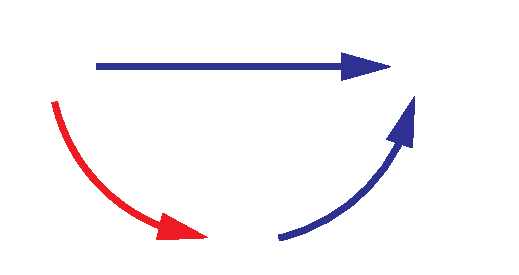
\includegraphics{Figures/Chapter1/decay_CMYK.pdf}%
\end{picture}%
\setlength{\unitlength}{4144sp}%
%
\begingroup\makeatletter\ifx\SetFigFont\undefined%
\gdef\SetFigFont#1#2#3#4#5{%
  \reset@font\fontsize{#1}{#2pt}%
  \fontfamily{#3}\fontseries{#4}\fontshape{#5}%
  \selectfont}%
\fi\endgroup%
\begin{picture}(3939,2094)(2644,-2188)
\put(3286,-736){\makebox(0,0)[rb]{\smash{{\SetFigFont{25}{30.0}{\sfdefault}{\mddefault}{\updefault}{\color[rgb]{0,0,0}$\Bs$}%
}}}}
\put(5761,-736){\makebox(0,0)[lb]{\smash{{\SetFigFont{25}{30.0}{\sfdefault}{\mddefault}{\updefault}{\color[rgb]{0,0,0}$\ffig$}%
}}}}
\put(4501,-421){\makebox(0,0)[b]{\smash{{\SetFigFont{25}{30.0}{\sfdefault}{\mddefault}{\updefault}{\color[rgb]{0,0,1}}%
}}}}
\put(5581,-1771){\makebox(0,0)[lb]{\smash{{\SetFigFont{25}{30.0}{\sfdefault}{\mddefault}{\updefault}{\color[rgb]{0,0,1}}%
}}}}
\put(3331,-1771){\makebox(0,0)[rb]{\smash{{\SetFigFont{25}{30.0}{\sfdefault}{\mddefault}{\updefault}{\color[rgb]{1,0,0}}%
}}}}
\put(4501,-2041){\makebox(0,0)[b]{\smash{{\SetFigFont{25}{30.0}{\sfdefault}{\mddefault}{\updefault}{\color[rgb]{0,0,0}$\Bsb$}%
}}}}
\end{picture}%
}
  \caption{The two interfering decay amplitudes leading to the same final state.
           The phases $\phimixfig$, $\phifig$ correspond to ....
           % This is assuming no CP violation in mixing or CP violation in decay.}
           }
  \label{interference}
\end{figure}

The parameter \phis manifests in the so called $\bquark \rightarrow \cquark\cquarkbar\squark $ transitions, where the
\bquark quuark of the \Bs meson decays into three other quarks. In addtion, the final state of the \Bs meson has to be
a CP eigenstate, which implies that both \Bs and \Bsb can decay into it, such that the two decay amplitudes of \figref{interference}
can interfere.

A common way to parametrize CP violation in the interference between mixing and decay is shown in \equref{lambda_cpv}
\footnote{This $\lambda_f$ is not to be confused with the $\lambda$ of the WOlfenstein Prametrization.}.

\begin{equation}
 \lambda_{f} = \eta_f \frac{q}{p} \frac{\bar{A}_f}{A_f}. % \equiv \left|\lambda_f\right| e^{i\phis}.
\label{lambda_cpv}
\end{equation}

\noindent The ratios $|\qoverp|$ and $|\nicefrac{A_f}{\bar{A}_{f}}|$ are ascociated to the mixing and decay parts of \figref{interference} respectivelly.
Whereas $\eta_f$ is the CP eigenvalue of the final state $f$ and can be either $+1$ or $-1$ corresponding to CP-even and CP-odd respectivelly.
The above parameter $\lambda_f$ is also releated to the $\Acp{\rm mix}$ and $\Acp{\rm dir}$, see section 4.2 of~\cite{DeBruyn-thesis}.
Given the so called {\it master equations}{\color{red} ref pdg} for the decay rates of a \Bs and \Bsb
to a final state $f$, the \CP asymmetry due to the interference between mixing and decay\footnote{assuming $|\qoverp|=1$ and $|\nicefrac{A_f}{\bar{A}_{\bar{f}}}| = 1$ consistet with {\color{red} ref for nocpv in mix and decay}.}
is shown in \equref{cpv_interf}

\newcommand{\half}{\frac{1}{2}}
\begin{equation}
  \Acp{\text{inter}}(t) = \frac{ - \Im(\lambda_f) \sin(\Delta m_s t)} {\cosh(\half \Delta\Gamma_s t) - \Re(\lambda_f)\sinh(\half\Delta\Gamma_s t)}.
\label{cpv_interf}
\end{equation}

\noindent It is intreasting to point out that according to \equref{cpv_interf} CP asymmetry can still be observed in the interference between decay and
mixing even if no CP-Violation occurs in both the mixing and decay. This is posible if the overal phase of $\lambda_f$ in \equref{lambda_cpv} is not zero.
The asymmetry of \equref{cpv_interf} can vanish at a particular point of time or for a given time interval. Because of that \equref{lambda_cpv} should not
be integrated over time when measuring \phis. Impling that the time interval between the production and decay of a \Bs (\Bsb) meson has to be
known\footnote{This interval is called {\it decay time}.}.

\begin{figure}[h]
  \centering
  {\sffamily \input{Figures/Chapter1/tree}}
  \caption{{\color{red} Fix this to look more like \figref{QuarkMixing} and put ckm elements on the vertices}. Explain tha this is called tree diagram}
  \label{bs2jpsiphi}
\end{figure}

Given a certain final state $f$ \equref{lambda_cpv} can be expresed as a combination of CKM elements and thus obtain the
Standard Model estimate of $\Im(\lambda_f)$. The two mesons $\jpsi$ and $\phi$ is a typical choice for $f$ for reasons that are
explained later in this section. The leading order diagrams for the \BsJpsiPhi decay and the \BBbarSyst mixing are
shown in \figref{bs2jpsiphi} and \figref{bs_box} repsectivelly. From those diagrams the ratios $\qoverp$ and $\nicefrac{A_f}{\bar{A}_{f}}$
can be read as shown in \equref{qoverp}\footnote{Here it has been used {\color{red} equation blah from pdg} } and \equref{af_afbar} repsectivelly.

\begin{equation}
 \frac{q}{p} = \frac{\Vtb^*\Vts}{\Vtb\Vts^*}
\label{qoverp}
\end{equation}

\begin{equation}
 \frac{\bar{A}_{\jpsi\phi}} {A_{\jpsi\phi}} = \frac{\Vcb\Vcs^*}{\Vcb^*\Vcs}
\label{af_afbar}
\end{equation}

\noindent Combining \equref{qoverp}, \equref{af_afbar} and using the $\beta_s$ angle definition frm \equref{bsAnglesDef} the imaginary part of
$\lambda_{f}$ of \equref{lambda_cpv} is can be computed, see \equref{phis_def}\footnote{Based on the fact that for a complex number's argument, $\argu{z}$ it is: $\argu{z^{-1}}=\argu{-z}=\argu{z^*}=-\argu{z}$}.

\begin{align}
  \centering
 \Im(\lambda_f) =& \eta_f\sin\parenthesis{ \argu{\frac{\Vtb^*\Vts}{\Vtb\Vts^*}} + \argu{\frac{\Vcb\Vcs^*}{\Vcb^*\Vcs}} } \nonumber \\
                =& \eta_f\sin\parenthesis{ \argu{\parenthesis{\Vtb^*\Vts}^2}    + \argu{\frac{1}{\parenthesis{\Vcb^*\Vcs}^2}} }
                = \eta_f\sin\parenthesis{  2 \; \argu{\frac{\Vtb^*\Vts}{\Vcb^*\Vcs}} } \nonumber \\
                =& \sin\parenthesis{-2\betas}
                \equiv \eta_f\sin\parenthesis{\phis}
 \label{phis_def}
\end{align}

\noindent An additional implication arises from the choice of the $\jpsi\phi$ as the final state.
Specifically due to the fact that the last particles have a non zero spin quantum number, their combined wavefunction
is not a pure cp eigenstate. The eigenvalue $\eta_f$ of the last wavefunction dependants on the total angular momentum
$l$ of the $\jpsi$ and $\phi$ mesons. This dependancy has to be taken into acount in \equref{phis_def} resulting in \equref{phis_jpsiphi_def}

\begin{equation}
 \Im(\lambda_{\jpsi\phi}) = (-1)^l\sin\parenthesis{\phis}
 \label{phis_jpsiphi_def}
\end{equation}

\subsection{Measuring \phis}
\label{measuring_phis}

The parameter \phis has been measuremed in the \lhcb experiment by analysing the decays of \BsJpsiPhi~\cite{phis-3fb-paper}.
The particular choise of the last final state, where \phiKK and \Jpsimumu, was to do with several reasons. First the high number
of selected \BsJpsiPhi decays available at \lhcb, roughly $90$k at the end of the \runtwo is an advantage. Second it is relatively easy
to select real $\phi$ over other mesons that decay to a $K^+K^-$ pair. This is due to the fact that the $\phi$ meson dominates the
$K^+K^-$ mass distribution within a window of about $\pm 70 \mevcc$ around its mass. The last allows for the analysis to be
independant\footnote{There is some residual dependance left, which is very similar to what is described in \secref{Kpi_Invariant_mass}. }
of the \mkk mass variable and thus much simpler. However an angular analysis, see \secref{Diferential_Decay_Rate} is necessary
to disentangle the odd and even CP components of the final state $\jpsi\phi$, as it became apparent in \equref{phis_jpsiphi_def}.
In addition, as it was already implied \phis can be correctly probed only when the time dependance of the \BsJpsiPhi decays is taken into
account\footnote{Specifically \phis is the amplitude of the $\ket{\Bs{}_{,H}}$ and $\ket{\Bs{}_{,L}}$ time distribution oscilations
mentioned in and shown in {\color{red} ref to something.} }.
Furthermore knowledge on wheather the final state $\jpsi\phi$ originated from a \Bs or a \Bsb is necessary since it
improves the sensitivity of the \phis measuremnt. The techinique used to deduce this information is called {\it flavour tagging}
and it complicates the analysis further\footnote{One should also take into acount the experimental effects such as angular and time efficiencies plus modeling the \lhcb detector's time resolution.}.

\begin{figure}[h]
  \begin{center}
    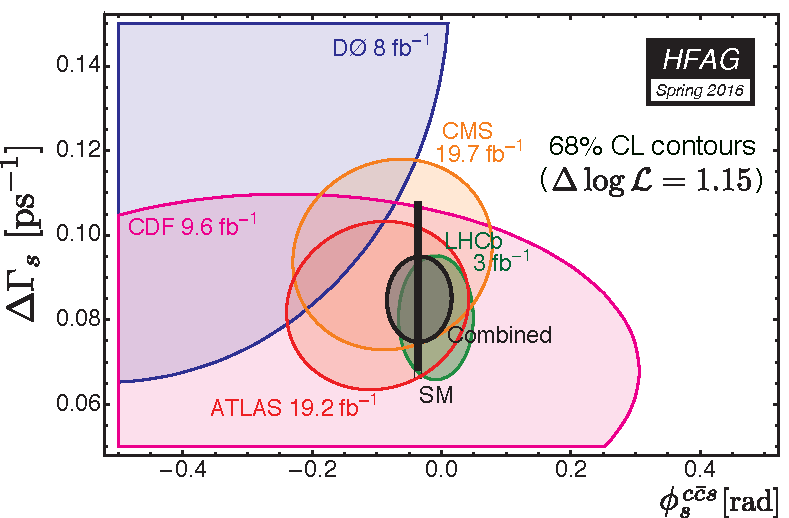
\includegraphics[trim=0cm 0cm 0cm 0cm, clip=true, scale=0.8]{Figures/Chapter1/hfag_Spring2016_DGsphis_zoom.pdf}
    \caption{Likelihood contours of $\Delta\Gamma-\phis$ (here $\phis\equiv \phis^{c\bar{cs}}$). Many individual measurements are
             combined to the black elipse. Standard Model prediction is represented by the black band. The \lhcb measurement
             mentioned in \equref{phis_lhcb} is illustrated by the green elipse. The combined measurements agree with the Standard Model
             predictions. Plot from \cite{hfag-2014} }
    \label{hfag_phis_dg}
  \end{center}
\end{figure}

\begin{subequations}
  \begin{equation}
  \centering
  \phiS{\lhcb}           =  -0.010 \pm 0.039(\text{total})  \;\; \text{rad}
  \label{phis_lhcb}
\end{equation}
\begin{equation}
  \phiS{SM,tree}  =  -2\betas = -0.03761 {}^{+0.00073}_{-0.00082}  \;\; \text{rad}
  \label{phis_theo}
\end{equation}
\end{subequations}

The status of the \phis measurements is shown in \figref{hfag_phis_dg}, where \lhcb has the most precise measurement to date.
The combined \phis value from the \lhcb experiment~\cite{phis-3fb-paper} is shown in \equref{phis_lhcb}.
The last is consistent with the Standard Model prediction of \equref{phis_theo}~\cite{ckm-fitter-phis-pred}\footnote{updated with summer 2015 result from the CKM-fitter group.}
 within the current experimental ucertainty.

\subsection{Probing New Physics}
\label{probe_new_phys}

{\color{red} consider citations fromt he jpsiKst paper.}

As it was explained at the end of \secref{The_Standard_Model} it seems that the Standard Model of particle physics needs to be extended
to describe effects and pehonomena beyond our current theoretical framework. In the majority of the Standard Model
extentions some new particle (field) is introduced, which is usually a new gauge boson or some symetry related
counter part of an existing particle. An example of the first could be the suggested $Z'$ {\color{red} ref}, hinted by
the recent \lhcb measuremnt. Whereas for the later {\it {Supersymetry}} {\color{red} ref to susy} doubles the
number of elementary particles by predicting a supersymetric version for each one of them.

There are typicaly two ways that those particles are sought for, namelly directly or inderctly. The first implies that the
assumed new particle is created in high energy physics colisions and its presentce is infered by detecting the products of
its decay. A typical example is the recent discovery of the higgs bosson at \lhc~\cite{higgs-cms,higgs-atlas}.
In the second scenario the presence of a new particle modifies some observable quantity, like $\phis$, in such a way that Standard Model
cannot explain. In that case it is not necessary for this partcile to be created in the first place.
One of the most significant examples of this type is the existance of the \tquark, which modified $\Bd-\Bdb$
oscilation fequency~\cite{argus-bbmix}. The second approach is the one that typical followed in flavor physics.

Particularly in the case of \BsJpsiPhi decays the predicted Standard Model value of \equref{phis_theo} is precise enough
such that the presence of new particles could shift its value ~\cite{Buras:2009if,Chiang:2009ev,Datta:2009fk} significantly.
Any deviation (small or large) is a direct evindence for physics beyond the Standard Model, making \phis an excelent observabale for probing NP.
This situation is shown in \equref{phis_meas} where the measured value \phiS{eff} is interpred
as the sum of the Standard Model prediction $\Delta\phiS{SM}$ and the intoduced from New Physics shift $\Delta\phiS{NP}$.

\begin{equation}
 \phis^{\text {eff}} = \phis^{\tiny \text{SM}} + \Delta\phiS{NP}
 \label{phis_meas}
\end{equation}

In view of the combined \phis result illustrated in \figref{hfag_phis_dg} New Physics effects must be small.
This is supported by other intreasting measuremnts of flavour physics observables where deviations from Standard Model are not significant enough
to claim the presence of New Physics effects. Such hints come from the rare decays $\Bmm$, $\BdKstmumu$ or from the \Vub CKM element
where different type of measurements exhibit tentions with each other that are not expected from the Standard Model.
An intreasting fact that could be helpfull in the future is that all those deviations and tentions are
corelated with each other. Meaning that under the assumption of a certain New Physics model all the falvor physics
observables need to from a consistent picture such that the assumed model can unambiguislly be identified.
The last points out also the power of flavour physics observables.

Lastly, the smallness of New Physics hints compels the scientific comunity to continue monitoring all the
flavor physics observables with higher precision, both from the theory and the experimental side.
However, in this increaed precision era higher order effects become importat which need to be taken into account,
as explained in see \secref{TheBsJpsiKstDecay}. Given that, \phis will most likely play an important role in the
pursuit for New Physics.

\subsection{Higher Order Effects in \phis}
\label{TheBsJpsiKstDecay}
As it was mentioned in \secref{WeakPhase} \BsJpsiPhi decays are dominated by the tree diagram of \figref{bs2jpsiphi}.
However the same decay could also take place via a higher order supressed process, for example the so called {\it penguin} diagram (or topology)
shown in \figref{bs2jpsiphi_peng}. The \phis measurement of \equref{phis_lhcb} ignores the contribution of the last penguing diagram.

\begin{figure}[h]
  \centering
  {\sffamily %%BoundingBox: -5 0 121 170
%%HiResBoundingBox: -5 0 120.57008 169.36447

\begin{fmffile}{Figures/Chapter1/penguin}
  \fmfframe(17,-25)(31,-25){
    \begin{fmfgraph*}(115,170)
      \fmfstraight
      \fmfleft{i0,i1,i2,i3,i4,i5}
      \fmfright{o0,o1,o2,o3,o4,o5}
      \fmf{fermion,tension=1.8,label.side=left,label=b}{v5,i3}
      \fmf{fermion,tension=1.5,right=0.2,label.side=left,label={\hspace*{18pt}u,,c,,t}}{v2,v5}
      \fmf{gluon,tension=2}{v4,v2}
      \fmf{dbl_dashes,tension=0}{v4,v2}
      \fmf{fermion,tension=0.3,right=0.2,label.side=left }{v3,v2}
      \fmf{boson,tension=0.6,left=0.3,label=W$^+$,label.side=left}{v3,v5}
      \fmf{fermion,label=c,tension=0.9,right=0.3,label.side=left}{o4,v4}
      \fmf{fermion,label=c,tension=0.9,right=0.3,label.side=left}{v4,o3}
      \fmf{fermion,label=s,label.side=left}{o2,v3}
      \fmffreeze
      \fmf{fermion,tension=0.7,label=s,label.side=left}{v1,o1}
      \fmf{fermion,tension=1,label.side=left,label=s}{i2,v1}
      %\fmf{phantom,tension=0.4}{v4,v1}
      \fmf{phantom,tension=0.4}{v3,v1,v5}
      \fmf{plain,right=0.2}{i2,i3}
      \fmf{plain,left=0.2,label=$\Bs$}{i2,i3}
      \fmf{plain,right=0.2,label=$\phi$}{o1,o2}
      \fmf{plain,left=0.2}{o1,o2}
      \fmf{plain,right=0.2,label=$\jpsi$}{o3,o4}
      \fmf{plain,left=0.2}{o3,o4}
    \end{fmfgraph*}
  }
\end{fmffile}
}
  \caption{{\color{red} Fix this to look more like \figref{QuarkMixing} and put ckm elements on the vertices}. Explain tha this is called tree diagram}
  \label{bs2jpsiphi_peng}
\end{figure}

\noindent This has been a reasonable assumtion before the \lhcb measurement which showed that the measured \phiS{eff} value is consistent with the Standard
Model prediction \phiS{SM,tree}, within the current experimental accuracy. However with increasing accuracy {\color{red} ref lhcb upgrade \phis sensitivy}
the last assumption needs to be revisited.
Specifically, because of the fact that penguin topology contributions shift the leading tree level Standard Model prediction.
The last shift could be misinterpreted as $\Delta\phiS{NP}$ if those penguin contributions are not properly esimated.
Thus in order to correctly probe New Physics contributions in fututre measurements the penguin topology contributions $\Delta\phiS{SM,peng}$
have to be estimated.

\begin{equation}
\phis^{\text {eff}} = \phis^{\tiny \text{SM,tree}} + \Delta\phiS{SM,peng} + \Delta\phis^{\tiny \text{NP}}
 \label{phis_sm_peng}
\end{equation}

\noindent The above situation is spelled out in \equref{phis_sm_peng}.
Calculations for the penguin contributions to $\Delta\phiS{SM,peng}$ are available {\color{red} 40 and 41 in kyrstofs thesis}.
However, these cacluations are difficult to perform, since they involve non-perturbative long-distance QCD effects. Thus an alternative
approach, according to {\color{red} krystof and rob}, is followed in order to experimentally extract $\Delta\phiS{SM,peng}$ by relying to
similar decay cahanells as \BsJpsiPhi as well. By doing so the presition on the penguin contributions increases. A desctription
of the necessesary formalism to extract the penguin shift, $\Delta\phiS{SM,peng}$, using also the chanells \BsJpsiKst and \BsJpsiRho is
given in \chapref{Penguins}.
